\section{Sesión 3}

\begin{definicion}
	La \textbf{oscilación} de una función acotada $f$ sobre un conjunto $A$ es $\operatorname{osc}_A(f):= \sup_A(f)-\inf_A(f)$. 
\end{definicion}

\begin{nota}
	Si $f:[a,b]\to\mathbb{R}$ es acotada, y si $P\in P[a,b]$, entonces: 
	$$U(P,f)-L(P,f)=\sum_{k=1}^{n}[M_k(f)-m_k(f)]\Delta x_k=\sum_{k=1}^{n}\operatorname{osc}_{I_k}(f)\Delta x_k$$
\end{nota}

\begin{prop}
	Suponga que $f,g:[a,b]\to \mathbb{R}$ son acotadas y suponga que $g\in R[a,b]$. Si $\exists c>0\ni \operatorname{osc}_I(f)\leq c\operatorname{osc}_I(g)$, sobre cada subintervalo $I\subseteq [a,b]$, entonces $f\in R[a,b]$. 
\end{prop}

\begin{teorema}
	$f\in R[a,b]$ ssi existe una sucesión de particiones $(P_n)$, $P_n\in P[a,b], \forall n\in \mathbb{Z}^+ \ni \lim_{n\to\infty}\left[U(f,P_n)-L(f,P_n)\right]=0$. En este caso, 
	$$\int_a^b f=\lim_{n\to \infty}U(f,P_n)=\lim_{n\to\infty}L(f,P_n).$$
\end{teorema}

\begin{teorema}
	Una función continua $f:[a,b]\to\mathbb{R}$ es Riemann integrable. 
\end{teorema}

\begin{teorema}
	Una función monótona $f:[a,b]\to\mathbb{R}$ es Riemann integrable. 
\end{teorema}

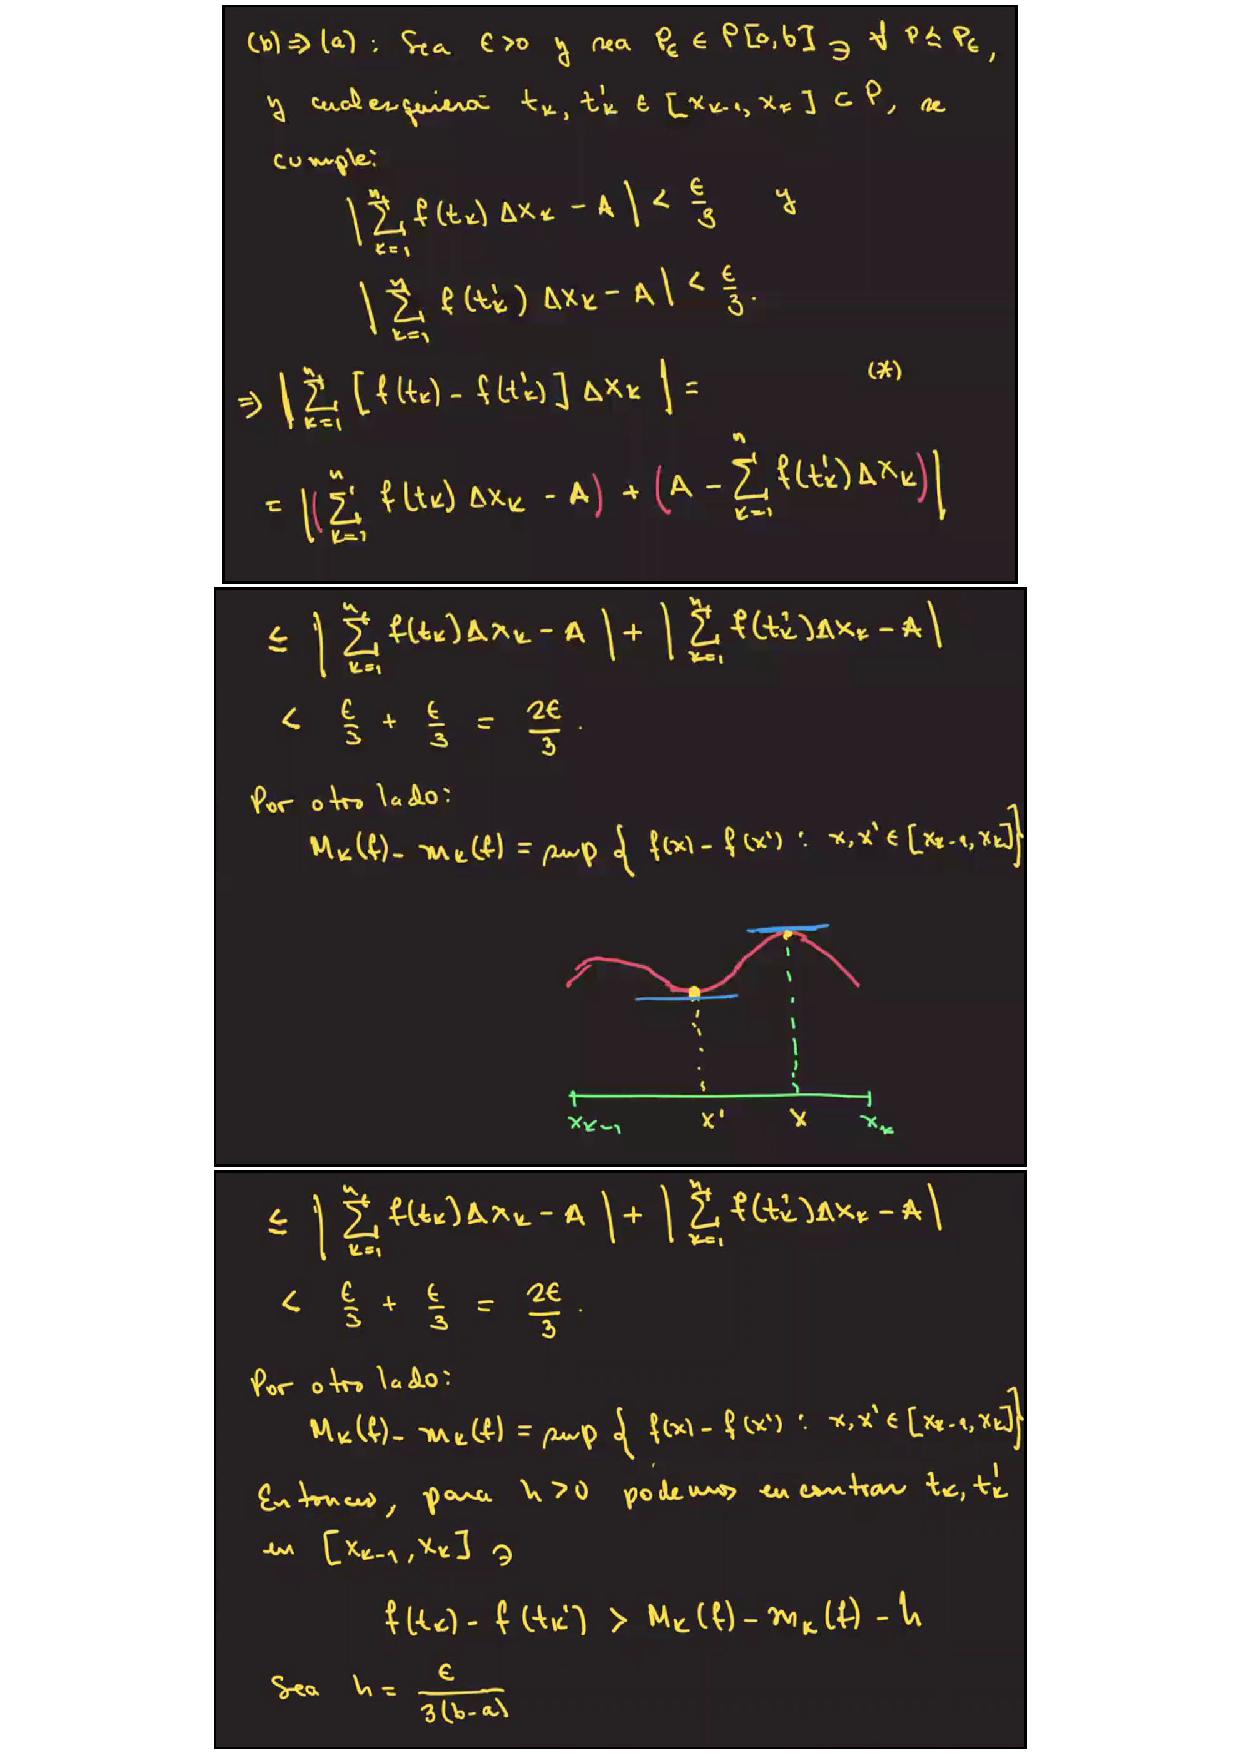
\includepdf[pages=-]{apendices/s3.pdf}